\subsubsection{Navegació pels resultats de diferents anys}

\paragraph{}
Aquesta funcionalitat, disposa d’una barra de navegació, que permeten canviar l’any sobre el qual els gràfics mostren informació. Aquesta barra, es troba a l’inici de la zona de resultats i es manté fixa i sobreposada als altres elements del HTML, si s’arriba a certa profunditat en la pàgina web.

Aquesta barra de navegació, cobreix un doble objectiu. En primer lloc, informar a l'usuari sobre a quin any pertanyen les dades dels gràfics pintats i en segon lloc, permetre la navegació a través de les dades dels diferents anys, si aquestes existeixen.

Les opcions per navegar a través dels gràfics de diferents anys, només es troben disponible si s'ha demanat dades per més d'un any. A més a més, s'ha dotat  d'intel·ligència als controls, per impedir l'accés a gràfics que no existeixen.

La imatge~\ref{fig:topFixed} mostra aquesta barra de control.

\begin{figure}[h]
    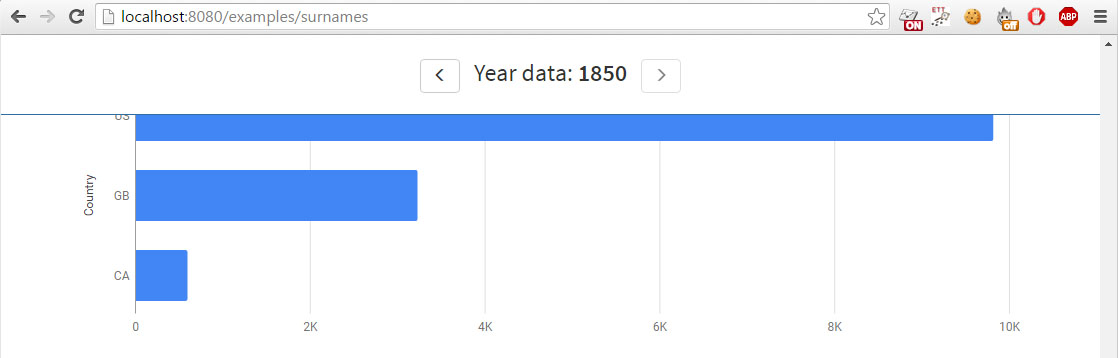
\includegraphics[width=\linewidth]{11/03_surnamesSearch/08_topFixed}
    \centering
    \caption{Barra de navegació pels gràfics de diferents anys}\label{fig:topFixed}
\end{figure}
